\documentclass{article}\usepackage[]{graphicx}\usepackage[]{xcolor}
% maxwidth is the original width if it is less than linewidth
% otherwise use linewidth (to make sure the graphics do not exceed the margin)
\makeatletter
\def\maxwidth{ %
  \ifdim\Gin@nat@width>\linewidth
    \linewidth
  \else
    \Gin@nat@width
  \fi
}
\makeatother

\definecolor{fgcolor}{rgb}{0.345, 0.345, 0.345}
\newcommand{\hlnum}[1]{\textcolor[rgb]{0.686,0.059,0.569}{#1}}%
\newcommand{\hlsng}[1]{\textcolor[rgb]{0.192,0.494,0.8}{#1}}%
\newcommand{\hlcom}[1]{\textcolor[rgb]{0.678,0.584,0.686}{\textit{#1}}}%
\newcommand{\hlopt}[1]{\textcolor[rgb]{0,0,0}{#1}}%
\newcommand{\hldef}[1]{\textcolor[rgb]{0.345,0.345,0.345}{#1}}%
\newcommand{\hlkwa}[1]{\textcolor[rgb]{0.161,0.373,0.58}{\textbf{#1}}}%
\newcommand{\hlkwb}[1]{\textcolor[rgb]{0.69,0.353,0.396}{#1}}%
\newcommand{\hlkwc}[1]{\textcolor[rgb]{0.333,0.667,0.333}{#1}}%
\newcommand{\hlkwd}[1]{\textcolor[rgb]{0.737,0.353,0.396}{\textbf{#1}}}%
\let\hlipl\hlkwb

\usepackage{framed}
\makeatletter
\newenvironment{kframe}{%
 \def\at@end@of@kframe{}%
 \ifinner\ifhmode%
  \def\at@end@of@kframe{\end{minipage}}%
  \begin{minipage}{\columnwidth}%
 \fi\fi%
 \def\FrameCommand##1{\hskip\@totalleftmargin \hskip-\fboxsep
 \colorbox{shadecolor}{##1}\hskip-\fboxsep
     % There is no \\@totalrightmargin, so:
     \hskip-\linewidth \hskip-\@totalleftmargin \hskip\columnwidth}%
 \MakeFramed {\advance\hsize-\width
   \@totalleftmargin\z@ \linewidth\hsize
   \@setminipage}}%
 {\par\unskip\endMakeFramed%
 \at@end@of@kframe}
\makeatother

\definecolor{shadecolor}{rgb}{.97, .97, .97}
\definecolor{messagecolor}{rgb}{0, 0, 0}
\definecolor{warningcolor}{rgb}{1, 0, 1}
\definecolor{errorcolor}{rgb}{1, 0, 0}
\newenvironment{knitrout}{}{} % an empty environment to be redefined in TeX

\usepackage{alltt}
\usepackage{amsmath} %This allows me to use the align functionality.
                     %If you find yourself trying to replicate
                     %something you found online, ensure you're
                     %loading the necessary packages!
\usepackage{amsfonts}%Math font
\usepackage{graphicx}%For including graphics
\usepackage{hyperref}%For Hyperlinks
\usepackage[shortlabels]{enumitem}% For enumerated lists with labels specified
                                  % We had to run tlmgr_install("enumitem") in R
\hypersetup{colorlinks = true,citecolor=black} %set citations to have black (not green) color
\usepackage{natbib}        %For the bibliography
\setlength{\bibsep}{0pt plus 0.3ex}
\bibliographystyle{apalike}%For the bibliography
\usepackage[margin=0.50in]{geometry}
\usepackage{float}
\usepackage{multicol}

%fix for figures
\usepackage{caption}
\newenvironment{Figure}
  {\par\medskip\noindent\minipage{\linewidth}}
  {\endminipage\par\medskip}
\IfFileExists{upquote.sty}{\usepackage{upquote}}{}
\begin{document}

\vspace{-1in}
\title{Lab 10 -- MATH 240 -- Computational Statistics}

\author{
  Jackson Colby \\
  Colgate University  \\
  Mathematics  \\
  {\tt jcolby@colgate.edu}
}

\date{}

\maketitle

\begin{multicols}{2}

\section{Introduction}
A polling company Gallup conducted a study on whether or not 1004 adults were satisfied or not with the postion of the United States. 39\% of respondents said they were satisfied and Gallup reported a $\pm$ 4\% margin of error. Gallup mentions that by increaseing the poll size to 2000, the results would be accurate within $\pm$ 2\%. This claim by Gallup is what leads us to the question for the lab, testing the claim of Gallup that increasing the sample size by double would decrease the margin of error by a half.

Utilizing packages such as tidyverse \citep{tidyverse} and ggplot2 \citep{ggplot2}, the following steps were conducted to test whether Gallup's method of calculating margin of error for their polls is correct. A basic simulation of two samples sizes n=1000 and n=2000 was conducted to see if the population value of 0.39 followed the claim of Gallup in their conducting of polls. Resampling was then used to find an approximation for \emph{p} hat to compare the margin of errors. To further test Gallup we then simulated of different n and \emph{p}, and finally calculated the actual margin of error using Wilson's Estimate.

\section{Basic Simulation}

This analysis compares the sampling distribution of sample proportions from 10,000 simulated polls at two different sample sizes: 1000 and 2000, assuming a true satisfaction rate of 39\%.

\begin{knitrout}
\definecolor{shadecolor}{rgb}{0.969, 0.969, 0.969}\color{fgcolor}
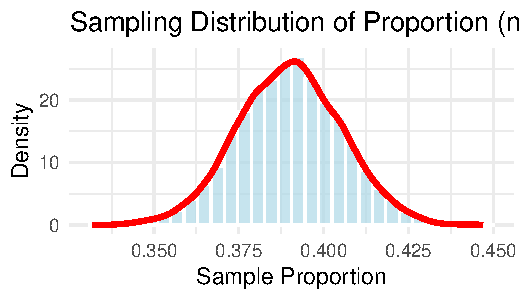
\includegraphics[width=\maxwidth]{figure/unnamed-chunk-1-1} 

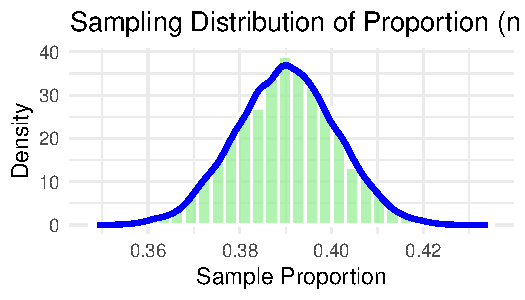
\includegraphics[width=\maxwidth]{figure/unnamed-chunk-1-2} 
\end{knitrout}

The shape of the sampling distribution for a sample size of 1000 forms an almost normal bell-shaped curve. The middle 95\% of the data fell between 0.36 and 0.42, meaning it had a margin of error of 0.03, which is slightly less than the 0.04 (4\%) that Gallup reported.

The shape of the sampling distribution for a sample size of 2000 also formed an almost normal bell-shaped curve. The data in this sample was a little bit more centralized around the assumed population mean. The middle 95\% of the data fell between 0.369 and 0.411, meaning it had a margin of error of 0.021, which is very close to the 0.02 (2\%) that Gallup reported.

\section{Resampling}

This analysis uses resampling to simulate the distribution of the sample proportion from a Gallup survey where 39\% of respondents are satisfied.

\begin{knitrout}
\definecolor{shadecolor}{rgb}{0.969, 0.969, 0.969}\color{fgcolor}
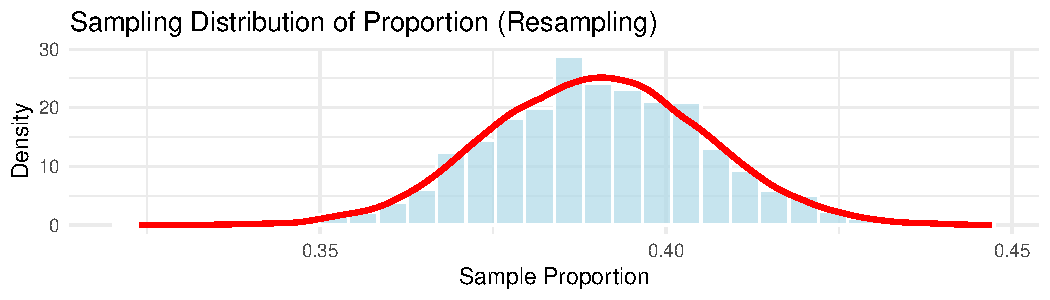
\includegraphics[width=\maxwidth]{figure/unnamed-chunk-2-1} 
\end{knitrout}

The resampling approach produced a normal bell shaped curve like the samples above, however the data fits the curve a little better than the basic simulation. The middle 95\% of the data fell between 0.36 and 0.42 leading to a margin of error of approximately 0.03, which is less than the 0.04 (4\%) that Gallup reported. This number is approximately the same number calculated from the data in the basic simulation for sample size of 1000. 

\section{Simulation over n and p}

This plot uses simulation to estimate the margin of error for different combinations of sample size ($n$) and true proportion ($p$), based on 10,000 binomial trials per combination.

\begin{knitrout}
\definecolor{shadecolor}{rgb}{0.969, 0.969, 0.969}\color{fgcolor}
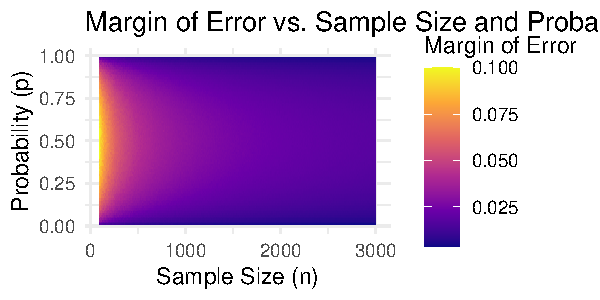
\includegraphics[width=\maxwidth]{figure/unnamed-chunk-3-1} 
\end{knitrout}

As seen in the figure above, Gallup mentioning the sample size as the sole factor in changing the margin of error is not completely true. The sample size does play a role in determining the margin of error, but the proportion \emph{p} also plays a role. When \emph{p} is close to the extremes (0 or 1) the margin of error is smaller for the same sample size. This is due to not being able to expand beyond the parameter space of [0,1].

\section{Actual Margin of Error}

This plot visualizes the margin of error for different combinations of sample sizes ($n$) and proportions ($p$), using the Wilson Margin of Error.

\begin{knitrout}
\definecolor{shadecolor}{rgb}{0.969, 0.969, 0.969}\color{fgcolor}
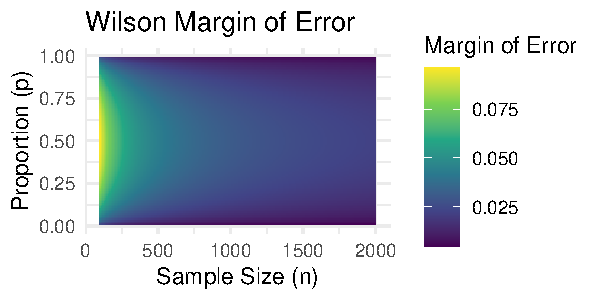
\includegraphics[width=\maxwidth]{figure/unnamed-chunk-4-1} 
\end{knitrout}

Similarly to the simulation over n and \emph{p}, the actual margin of error using the Wilson Estimare paints a similar picutre. The plots follow a similar pattern, ultimately showing that Gallup's story is not as straightforward as they mention. The sample size does decrease the margin of error as n increases, however \emph{p} also plays a factor in the margin of error. Similarly to before the values of \emph{p} closer to the extremes of 0 and 1 have lower margin of errors since the values can not go outside the parameter space of [0,1].

\section{Results}
Wilson's claim that doubling the sample size from 1000 to 2000 would decrease the margin of error from $\pm$ 4\% to $\pm$ 2\% is not as simple as they claim. This is primarily shown from the Simulation over n and \emph{p} and the Actual Margin of Error Calculation utilizing Wilson's Estimate. The sample size is not the only factor in determining the margin of error, the proportion \emph{p} also playing a role. This suggests that Gallup's claim is not true, or at a minimum it is not true for all values of \emph{p}.


\begin{tiny}
\bibliography{bib}
\end{tiny}
\end{multicols}



\end{document}
